\documentclass[11pt,fleqn]{article} % Default font size and left-justified equations

%\usepackage{standalone}

\usepackage{todonotes}
\usepackage{color}
% use \todo{note} OR \missingfigure{Add my picture here}

\usepackage[top=3cm,bottom=3cm,left=3.2cm,right=3.2cm,headsep=10pt,a4paper]{geometry} % Page margins
\usepackage{xcolor} % Required for specifying colors by name
\definecolor{ocre}{RGB}{243,102,25} % Define the orange color used for highlighting throughout the book


% Font Settings


% SLG commented out


% \usepackage{avant} % Use the Avantgarde font for headings
%\usepackage{times} % Use the Times font for headings
% \usepackage{microtype} %Slightly tweak font spacing for aesthetics
% \usepackage{mathptmx} % Use the Adobe Times Roman as the default text font together with math symbols from the Sym­bol, Chancery and Com­puter Modern fonts


%  \usepackage[scaled=0.90]{couriers} %What is this used for?




% SLG commented out
% \def\thereforesymbol{
% \leavevmode
% \lower0.1ex\hbox{$\cdot$}
% \kern-0.2em\raise0.7ex\hbox{$\cdot$}
% \kern-0.2em\lower0.2ex\hbox{$\cdot$}
% \thinspace}


% \usepackage{CJKutf8}
%For cyrillic characters  (do we have any?)


% slg commented this out:
% \usepackage[OT2,T1]{fontenc}
% \DeclareSymbolFont{cyrletters}{OT2}{wncyr}{m}{n}
% \DeclareMathSymbol{\Sha}{\mathalpha}{cyrletters}{"58}


\usepackage[T1]{fontenc}
\usepackage[section]{placeins}

% slg commented these out:
% \usepackage{amssymb}
 \usepackage{fancyvrb}
%  \usepackage{color}




%define a verbatim text for bold user input
\newcommand\verbbf[1]{\textbf{$\blacksquare$ #1}}
%define a verbatim text without box in front
\newcommand\verbbnbf{\textbf}


\PassOptionsToPackage{hyphens}{url}


\usepackage[pdftitle={Programmers Manual for Developing Bulk Extractor Scanner Plug-ins},
              pdfauthor={Jessica R. Bradley, Simson L. Garfinkel},
              pdfkeywords={bulk extractor, scanners, plug-ins, bulk extractor developers}]{hyperref}
\makeatletter
\g@addto@macro{\UrlBreaks}{\UrlOrds}
\makeatother
% \usepackage{microtype} % Slightly tweak font spacing for aesthetics
%\usepackage[utf8]{inputenc} % Required for including letters with accents
\usepackage[T1]{fontenc} % Use 8-bit encoding that has 256 glyphs




%\usepackage[a4paper,pdftex]{geometry}                                                                                % A4paper margins
\setlength{\oddsidemargin}{5mm}                                                                                                % Remove 'twosided' indentation
\setlength{\evensidemargin}{5mm}


\usepackage[english]{babel}
%\usepackage[protrusion=true,expansion=true]{microtype}        
\usepackage{amsmath,amsfonts,amsthm,amssymb}
\usepackage{graphicx}


\usepackage{tabularx}


% Simson commented this out:
%use autoref or Autoref for lowercase or uppercase beginning of references
\usepackage{catoptions}
\makeatletter
\def\figureautorefname{figure}
\def\tableautorefname{table}
\def\Autoref#1{%
  \begingroup
  \edef\reserved@a{\cpttrimspaces{#1}}%
  \ifcsndefTF{r@#1}{%
    \xaftercsname{\expandafter\testreftype\@fourthoffive}
      {r@\reserved@a}.\\{#1}%
  }{%
    \ref{#1}%
  }%
  \endgroup
}
\def\testreftype#1.#2\\#3{%
  \ifcsndefTF{#1autorefname}{%
    \def\reserved@a##1##2\@nil{%
      \uppercase{\def\ref@name{##1}}%
      \csn@edef{#1autorefname}{\ref@name##2}%
      \autoref{#3}%
    }%
    \reserved@a#1\@nil
  }{%
    \autoref{#3}%
  }%
}
\makeatother


\usepackage{amsmath}


\usepackage{booktabs}


% slg commented out:
% \usepackage{makecell}


\usepackage{color}
\usepackage{graphicx}
%\usepackage {hyperref}
\usepackage{listings}
\usepackage{xspace}


% slg commented out:
\usepackage[toc, page]{appendix}
\usepackage[labelfont=bf]{caption}
%http://tex.stackexchange.com/questions/27663/using- bold-italic-text-inside-listings


% slg commented out:
% \usepackage{multirow} %for multirow tables




\newcommand{\HRule}{\rule{\linewidth}{0.5mm}}
\usepackage{fancyhdr}


\usepackage{array}



\setcounter{secnumdepth}{5}
\setcounter{tocdepth}{5}
 
%\usepackage{arabtex}

\usepackage{verbatim}

\raggedbottom

\begin{document}

%define macros for commonly used terms that require special formatting
\newcommand \sscope {\textit{SectorScope}\xspace}
\newcommand \hdb {\textit{hashdb}\xspace}
\newcommand \aut {\textit{Autopsy}\xspace}
\newcommand \bulk {\textbf{bulk\_extractor}\xspace}
\newcommand \mdd {\textbf{md5deep}\xspace}
\newcommand \fiwalk {\textbf{fiwalk}\xspace}

\hypersetup{%
    pdfborder = {0 0 0}
}

\lstdefinestyle{customfile}{
basicstyle=\footnotesize\ttfamily, frame=single, float=htpb}

\begin{titlepage}





% LaTeX Template: Titlepage
% This is a title page template which be used for both articles and reports.
%
% Copyright: http://www.howtotex.com/
% Date: April 2011
% ------------------------------------------------------------------------------

% -------------------------------------------------------------------------------
% Preamble
% -------------------------------------------------------------------------------
%\documentclass[paper=a4, fontsize=11pt,twoside]{scrartcl}		% KOMA article


% ------------------------------------------------------------------------------
% Definitions (do not change this)
% ------------------------------------------------------------------------------
\newcommand{\TRule}[1]{\rule{\linewidth}{#1}} 	% Horizontal rule

\makeatletter							% Title
\def\printtitle{%						
    {\centering \@title\par}}
\makeatother									

\makeatletter							% Author
\def\printauthor{%					
    {\centering \large \@author}}				
\makeatother							

% ------------------------------------------------------------------------------
% Metadata (Change this)
% ------------------------------------------------------------------------------
\title{	\LARGE \textsc{\textit{SectorScope}} 	% Subtitle of the document
		 	\\[1.0cm]													% 2cm spacing
			\TRule{0.5pt} \\										% Upper rule
			\LARGE \textbf{\uppercase{Users Manual}}	% Title
			\TRule{2pt} \\ [0.5cm]								% Lower rule + 0.5cm spacing
			%\small \textit{Quickstart Guide Included}\\
			\normalsize \today									% Todays date
		}
\author{
		Authored by: \\
		Bruce D. Allen\\
}

% ------------------------------------------------------------------------------
% Maketitle
% ------------------------------------------------------------------------------
\thispagestyle{empty}				% Remove page numbering on this page

\printtitle									% Print the title data as defined above
  	\vfill
\printauthor								% Print the author data as defined above














\end{titlepage}


\pagenumbering{roman}
\setlength{\parindent}{0pt} %remove indenting from whole document
\newpage
\thispagestyle{empty}
\mbox{}
\newpage


\section{Introduction}
\subsection {Overview of \sscope}
\sscope is a graphical interface tool for viewing blocks that match blacklist block hashes stored in a \hdb database. \sscope includes interfaces for scanning media images, ingesting source files into \hdb databases, and directly viewing raw media image bytes.\\

\subsection{Obtaining \sscope}
\label{Obtaining}
\sscope requires \hdb. Both tools are readily available for Windows systems, Linux flavors, and MacOS.  A Windows installer is available for Windows users.  A source code distribution is available for Linux and Mac users.  Developers may download these tools directly from source available on GitHub.\\

\subsubsection{Installing on Windows}
Download and run the latest \sscope Windows installer available under \url{https://github.com/NPS-DEEP/NPS-SectorScope/blob/master/build}. Click on the latest \verb+.exe+ file, click on \verb+View Raw+, save it, and then run that.\\

\hdb is available under \url{http://digitalcorpora.org/downloads/hashdb}. Please see \hdb documentation for further information on installing \hdb.\\

\subsubsection{Installing on Linux or Mac}
Download and unzip \sscope files from the \verb+.zip+ file under \url{https://github.com/NPS-DEEP/NPS-SectorScope/blob/master/build}.\\ Please see \url{https://github.com/NPS-DEEP/hashdb/wiki/Installing-hashdb} for information on installing \hdb.\\

\section{Using \sscope}
\subsection{Starting \sscope}
\begin{itemize}
\item Type \verb+sectorscope.py+. Type \verb+sectorscope.py -h+ for help on options.
\item In \aut, click the \verb+SectorScope+ property.
\end{itemize}

\subsection{Main Window}
Here is an example screenshot of the \sscope main window:\\
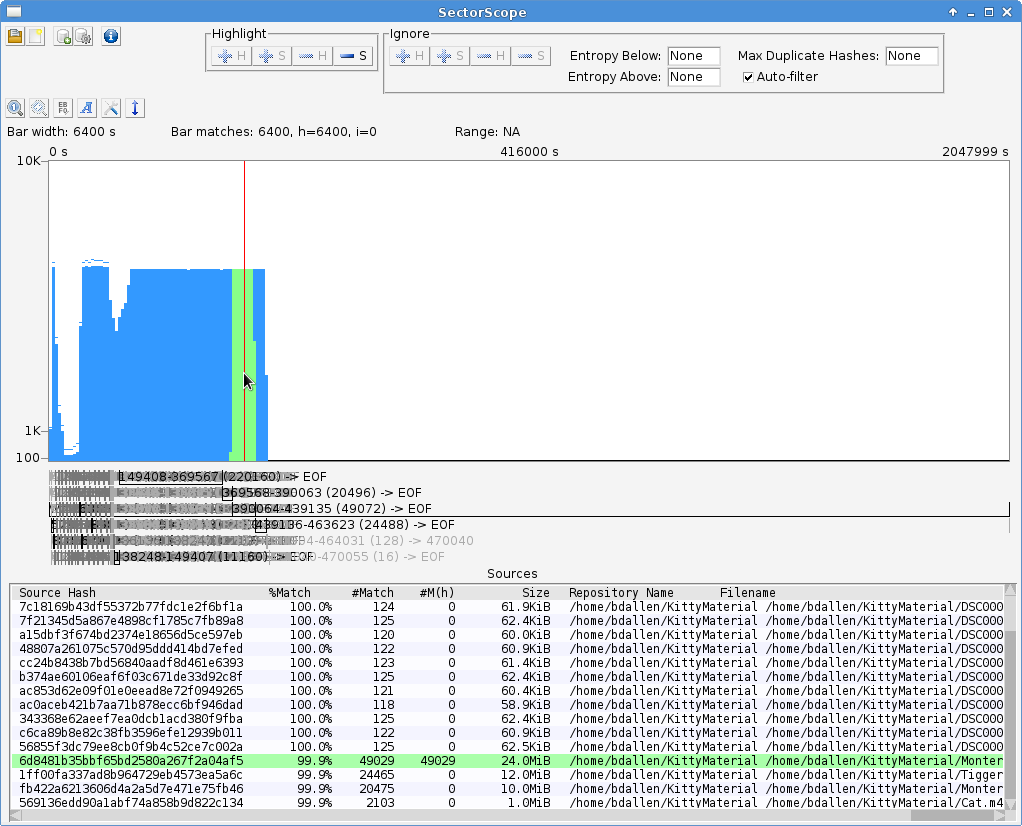
\includegraphics[scale=.4]{screenshots/main_window}\\

\subsection{Menu Controls}
Here are the menu controls:\\
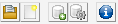
\includegraphics[scale=.4]{screenshots/menu_controls}\\

\subsubsection{Open Scan File}
Here is the Open Scan File window:\\
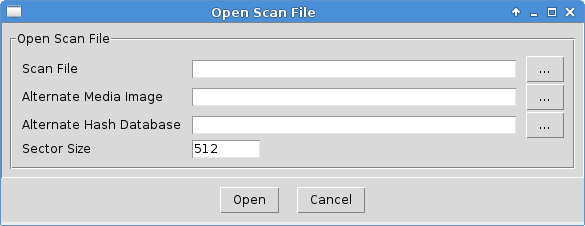
\includegraphics[scale=.4]{screenshots/open_scan_file}\\
\begin{itemize}
\item \textbf{Scan File}\\
When \hdb performs a scan, all matches are placed in this scan file. The scan file also contains the path to the media image scanned and the hash database scanned against. If these paths move, alternate paths may be provided.
\item \textbf{Alternate Media Image}\\
An alternate path to the media image to use if the path in the scan file is incorrect. Keep blank to use the default.
\item \textbf{Alternate Hash Database}\\
An alternate path to the hash database to use if the path in the scan file is incorrect. Keep blank to use the default.
\item \textbf{Sector Size}\\
The sector size for this media, typically 512 bytes. \sscope will display sectors of this size. \sscope will zoom in to this size.
\end{itemize}

\subsubsection{Scan Statistics}
Here is an example of scan statistics:\\
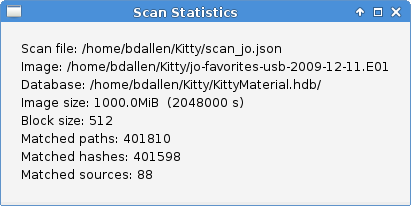
\includegraphics[scale=.4]{screenshots/scan_statistics}\\
Statistics for the opened scan include the path to the scan file, media image, and hash database, the image size, block size, and number of matched paths, hashes, and sources.

\subsubsection{Ingest}
Here is the \sscope Ingest window:\\
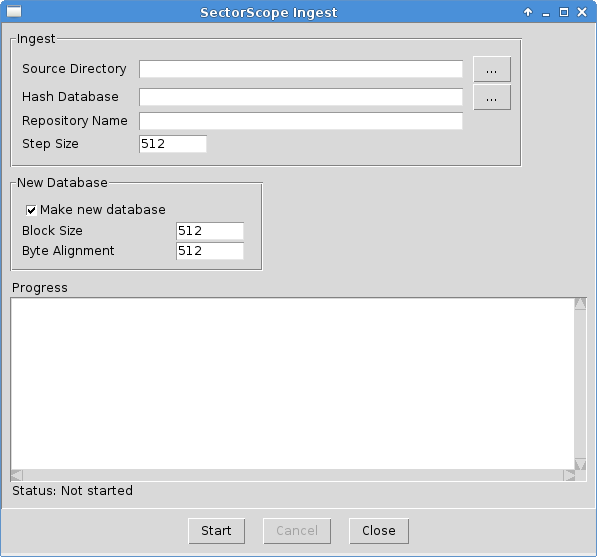
\includegraphics[scale=.4]{screenshots/ingest}\\
Use this window to ingest files or media images into a hash database.
\begin{itemize}
\item \textbf{Source Directory}\\
The path to the source files to ingest recursively from.
\item \textbf{Hash Database}\\
The path to the hash database to import block hashes into.
\item \textbf{Repository Name}\\
The repository name to associate the imported sources with. Leave blank to use the default, which is the source directory path.
\item \textbf{Step Size}\\
The step size to move along while calculating block hashes. The byte alignment must be compatible with the step size, specifically, byte alignment must be divisible by step size.
\item \textbf{Make New Database}\\
If this is selected, a new database will be created instead of using an existing databases. The new database will be created with the following:
  \begin{itemize}
  \item \textbf{Block Size}\\
  The block size to use for calculating the block hash.
  \item \textbf{Byte Alignment}\\
  An optimization parameter, typically the smaller of the block size and the step size.
  \end{itemize}
\end{itemize}

\subsubsection{Scan}
Here is the \sscope Scan Image window:\\
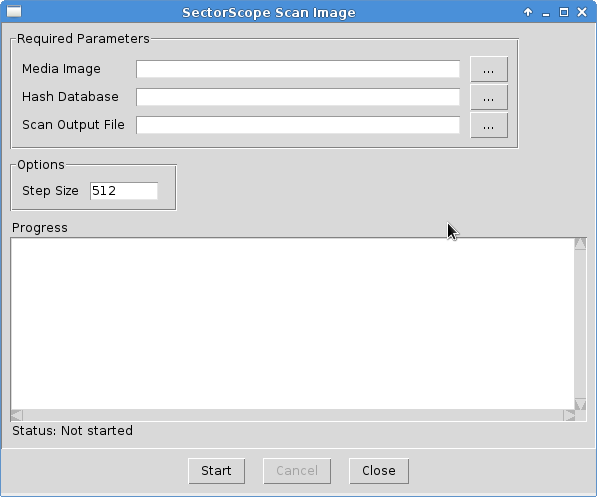
\includegraphics[scale=.4]{screenshots/scan}\\
Use this window to scan a media image for matching block hashes.
\begin{itemize}
\item \textbf{Media Image}\\
The path to the media image to scan.
\item \textbf{Hash Database}\\
The path to the hash database to scan against.
\item \textbf{Sector Size}\\
The sector size for this media, typically 512 bytes. \sscope will display sectors of this size. \sscope will zoom in to this size.
\end{itemize}

\subsubsection{Toggle Offset Units}
\sscope displays offsets as sectors, decimal bytes, or hexadecimal bytes. This button toggles the offset units across these view modes.

\subsubsection{Information}
This button opens a window showing the version of \sscope and \hdb.

\subsection{Highlight and Ignore}
Here is an example view of the highlight and ignore controls:\\
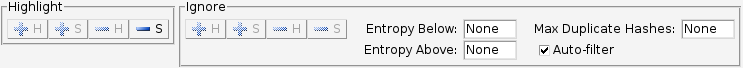
\includegraphics[scale=.4]{screenshots/highlight_and_ignore}\\
These buttons provide control over which hashes and sources are highlighted or ignored. Highlighted items are shown in green. Ignored items are not displayed.
\subsubsection{Highlight}
\begin{itemize}
\item \textbf{+H}\\
Select a range and highlight hashes in this range.
\item \textbf{+S}\\
 Select a range and highlight all sources containing hashes in this range.
\item \textbf{-H}\\
Un-highlight all highlighted hashes.
\item \textbf{-S}\\
Un-highlight all sources.
\end{itemize}

\subsubsection{Ignore}
\begin{itemize}
\item \textbf{Max Duplicate Hashes}\\
Ignore hashes matched more than a maximum number of times.
\item \textbf{Auto-filter}\\
Ignore hashes if they have been flagged as potentially non-probative based on experimental entropy calculations.
\item \textbf{+H}\\
Select a range and ignore hashes in this range.
\item \textbf{+S}\\
Select a range and ignore all sources containing hashes in this range.
\item \textbf{-H}\\
Stop ignoring all ignored hashes.
\item \textbf{-S}\\
Stop ignoring all ignored sources.
\end{itemize}






The step size to move along while calculating block hashes. The byte alignment must be compatible with the step size, specifically, byte alignment must be divisible by step size.

The repository name to associate the imported sources with. Leave blank to use the default, which is the source directory path.
\end{itemize}



An alternate path to the hash database to use if the path in the scan file is incorrect. Keep blank to use the default.


When \hdb performs a scan, all matches are placed in this scan file. The scan file also contains the path to the media image scanned and the hash database scanned against. If these paths move, alternate paths may be provided.



information about the media image containsis a scan file created from a \hdb scan. All block hashes that matched a scan are 


\begin{itemize}
\item The top-middle part of the view shows that the Block Match Viewer is displaying block matches in the 1GiB disk image \verb+jo-favorites-usb-2009-12-11.E01+ matching source files in hashdb image \verb+kitty_blacklist.hdb+.
\item: The \textbf{Filters} section at the top-left show:
  * There is no filtering applied to duplicate hashes.  For example if this value were 20, then block hash values that are cited from more than 20 sources would be filtered, meaning that these matches would not show up in the **Filtered matches removed** view and would show up in the **Filtered matches only** view.
  * Flagged blocks are marked as filtered.  You can turn off this filtering by turning off the checkmark.  The *bulk_extractor* *hashdb* scanner automatically flags blocks that are considered low entropy when hashes are imported.
* The middle-left portion of the viewer shows the **Image Match Histogram**.
  * Three histogram views are shown:
    * **All matches** shows a histogram of matches across the media image.
    * **Filtered matches removed** shows matches with filtered matches removed.
    * **Filtered matches only** shows the histogram of filtered matches.  Adjust filtering to adjust these histograms.
  * The vertical bar in the **Image Match Histogram** shows that an image offset has been selected, in this case, 0x03200000 hexadecimal or 52428800 decimal byte offset in the media image.  The raw bytes of this offset is shown below in the **Image Hex View**.
  * Zoom in all the way to individual sectors or zoom out to the whole media image view by moving the cursor over your desired zoom point and rolling the mouse wheel to your desired resolution.  Move the mouse to the right or left to change the zoom point.  The leftmost and rightmost sector offsets are shown just below the histogram window.
* The bottom-left portion of the viewer shows the **Image Hex View**.  Click on a a point in the histogram view to select a media image sector and its raw hex bytes will be shown here.  Also, the block hash will be shown.  If the block hash is matched by a source, you may filter the selected hash:
  * Click Add to filter the hash.  You may turn off all other filters to see where in the disk image that a particular hash resides.
  * Click Remove to remove the hash from the filter.

* The right side of the viewer shows **Matched Sources**.  This consists of a list of every source in the database that had hash blocks that matched the media image scanned.
  * Each source is shown in a row describing the following:
    * The source index, with a checkbox.  Select the checkbox to filter the associated source.
    * **%Match** The percent of sectors that the source has that were found in the media image.
    * **#Match** The number of sectors that the source has that were found in the media image.
    * **Size** The size, in bytes, of the source file.
    * **Repository** The repository name assigned to the source.
    * **File** The filename of the source.
  * Press the **Clear All** button to clear all source filters selected.  Press the **Select All** button to select them all.  Click on individual source checkboxes to filter individual sources.  For example turn off all filters except one source filter to see where in the media image that all hashes associated with a source are located.

### A note on filters
There are several filter types and they may be used by themselves or in combination with others:
* **Max Same Hashes** filters filter duplicate hashes.
* **Filter Flagged Blocks** filters hashes that have been flagged by the *bulk_extractor* *hashdb* scanner as having low entropy.
* **Block Hash Filters** filter hashes that have been selected individually.
* **Source Filters** filter hashes associated with specific sources.









































































\subsection{Menu Controls}
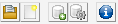
\includegraphics[scale=.8]{screenshots/menu_controls}



# Menu Controls
[[https://raw.githubusercontent.com/NPS-DEEP/NPS-SectorScope/master/doc/sectorscope_um/screenshots/menu_controls.png]]

* Open new project by providing a *bulk_extractor* scan directory.
* View properties about an opened project.
* Import a directory of files into a new *hashdb* database.
* Scan a media image for matches in a *hashdb* database.
* Toggle the offset value view between hexadecimal, decimal, or sector number.

# Highlighting Hashes and Sources
[[https://raw.githubusercontent.com/NPS-DEEP/NPS-SectorScope/master/doc/sectorscope_um/screenshots/highlight_controls.png]]
* `+H` Select a range and highlight hashes in this range.
* `+S` Select a range and highlight all sources containing hashes in this range.
* `-H` Un-highlight all highlighted hashes.
* `-S` Un-highlight all sources.

# Ignoring Duplicates, Low Entropy, Hashes, and Sources
[[https://raw.githubusercontent.com/NPS-DEEP/NPS-SectorScope/master/doc/sectorscope_um/screenshots/ignore_controls.png]]
* `Max Duplicate Hashes` Ignore hashes matched from more than a maximum number of sources.
* `Auto-filter` Ignore hashes if they have been flagged as potentially non-probative based on experimental entropy calculations.
* `+H` Select a range and ignore hashes in this range.
* `+S` Select a range and ignore all sources containing hashes in this range.
* `-H` Stop ignoring all ignored hashes.
* `-S` Stop ignoring all ignored sources.

# Histogram
[[https://raw.githubusercontent.com/NPS-DEEP/NPS-SectorScope/master/doc/sectorscope_um/screenshots/bar.png]]
The histogram view shows the frequency of hash matches at given offsets in the media image.
Frequency is distributed across about 300 buckets and is graphed as vertical bars.
Bars are colored blue.  If hashes are ignored, a blue tick is shown indicating frequency, instead of a bar.
Highlighted bars are colored green.
When selecting a range, the range is shaded light blue.

Use the mouse to navigate:

* Move the mouse to hover over a bar.
* Click and drag to select a range.  Click to unselect a range.
* Right-click and drag to pan.
* Roll the wheel to zoom in and out.

# Histogram Controls
[[https://raw.githubusercontent.com/NPS-DEEP/NPS-SectorScope/master/doc/sectorscope_um/screenshots/bar_controls.png]]

* Zoom to full scale.
* Zoom to range selection.
* Show a hex dump of a region within a range selection.
* Manage annotations about regions of the image such as volume metadata, associated filenames, etc, this capability is currently not implemented and is expected to be incrementally introduced.
* Increase or decrease the vertical scale by a factor of ten to rescale tall or short bars.

# Histogram Annotation
[[https://raw.githubusercontent.com/NPS-DEEP/NPS-SectorScope/master/doc/sectorscope_um/screenshots/bar_annotation.png]]
* `Bar width` The amount of the media image that one bar spans.
* `Bar matches` The amount of matches under the bar that the cursor is hovering over.  Three values are shown: total matches, highlighted matches (h), and ignored matches (i).
* `Range` The amount of the media image that the selected range spans.
* The first and last offset across the histogram is shown.
* The horizontal scale is shown, indicating the number of hash matches required to reach that height.

# Source Table
[[https://raw.githubusercontent.com/NPS-DEEP/NPS-SectorScope/master/doc/sectorscope_um/screenshots/sources_excerpt.png]]
Here are some properties of the source table:

* If a range is selected, only sources with hashes in that range are shown.  Otherwise, all hashes are shown.
* If all hashes of a source are ignored, that source will not be shown.
* Click on a source row to highlight that source.  Click again to un-highlight it.

Source rows contain the following information:

* The source ID, an internal index *hashdb* uses to reference a given source.
* `%Match` The percent of this source that was matched by the scan.
* `#Match` The number of matches matched by the scan.
* `#M(h)` The number of matches that are highlighted.
* `Size` The size of the source file matched.
* `Repository Name` The Repository name given to the source imported.
* `Filename` The filename given to the source imported.

\end{document}
